\section{Process perspective} \label{pp}

\subsection{Stages and tools in CI/CD} 
We have 3 pipelines that are triggered by various events in our  version control system:
\begin{itemize}
    \item Committing to feature/bugfix branch.
    \item Merging pull request from feature-branch to develop-branch.
    \item Merging the develop-branch into the main-branch.
\end{itemize}
Furthermore, we have set up some rules for protecting the main-branch.

\subsubsection*{Feature/working-branches}
The workflow shown in Figure \ref{fig:test-workflow} is triggered on every commit, and the status check is used to decide whether a PR to develop/main can be merged.
\begin{figure}[h!]
  \centering 
  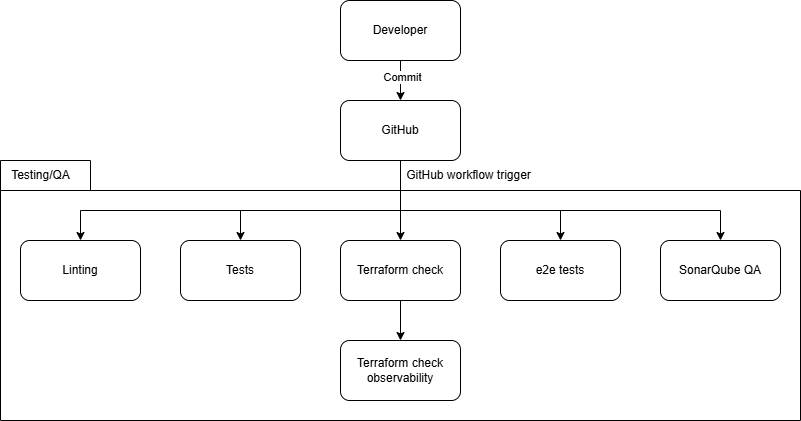
\includegraphics[width=\textwidth]{images/Testing workflow.png}
  \caption{Testing workflow}
  \label{fig:test-workflow}
\end{figure}

\subsubsection*{Merging PR into develop-branch}
A merge into this branch triggers a build with DEV environment variables, which is then deployed to our development environment.

\subsubsection*{Merging PR into main-branch}
The workflow triggered by a merge into the main-branch is almost the same as when merging into the development-branch. A build is made with production environment variables, and it is deployed to our PROD environment. When a new release is successfully deployed, a release is made on GitHub.

\subsubsection*{GitHub rule sets}
We have 3 rules specified on GitHub to secure against potentially broken, as a release is made whenever anything is merged into main. 

\begin{itemize}
    \item The first rule is that it is only possible to merge into main from the development-branch. This is done such that our automatic tests cannot be circumvented.
    \item The second is that pull-requests are only allowed to be merged into develop if all of our tests pass.
    \item The final rule is that it is not allowed to commit directly to our main- or develop-branch, but instead always require a pull-request, such that the correct workflows are triggered.
\end{itemize}
\subsection{Monitoring}
 Our monitoring efforts were displayed in Grafana, as can be observed in Figure \ref{fig:monitor}.
\subsubsection{Metrics}
Our metrics collection was done using the web-scraper Prometheus, which collects metrics from the MiniTwit endpoint “/metrics”. The metric endpoint was set up using the \texttt{ginprom} package in Go, which seamlessly integrates with \texttt{gin}, providing a multitude of information about the state of the MiniTwit app, \texttt{gin}, and Go runtime. Prometheus maintains its own storage locally, and to ensure that replacing the virtual machine does not lose its time series data, we created a dedicated volume in Digital Ocean to store this data, alongside the configuration files for Prometheus. 

\begin{figure} [H]
    \centering
    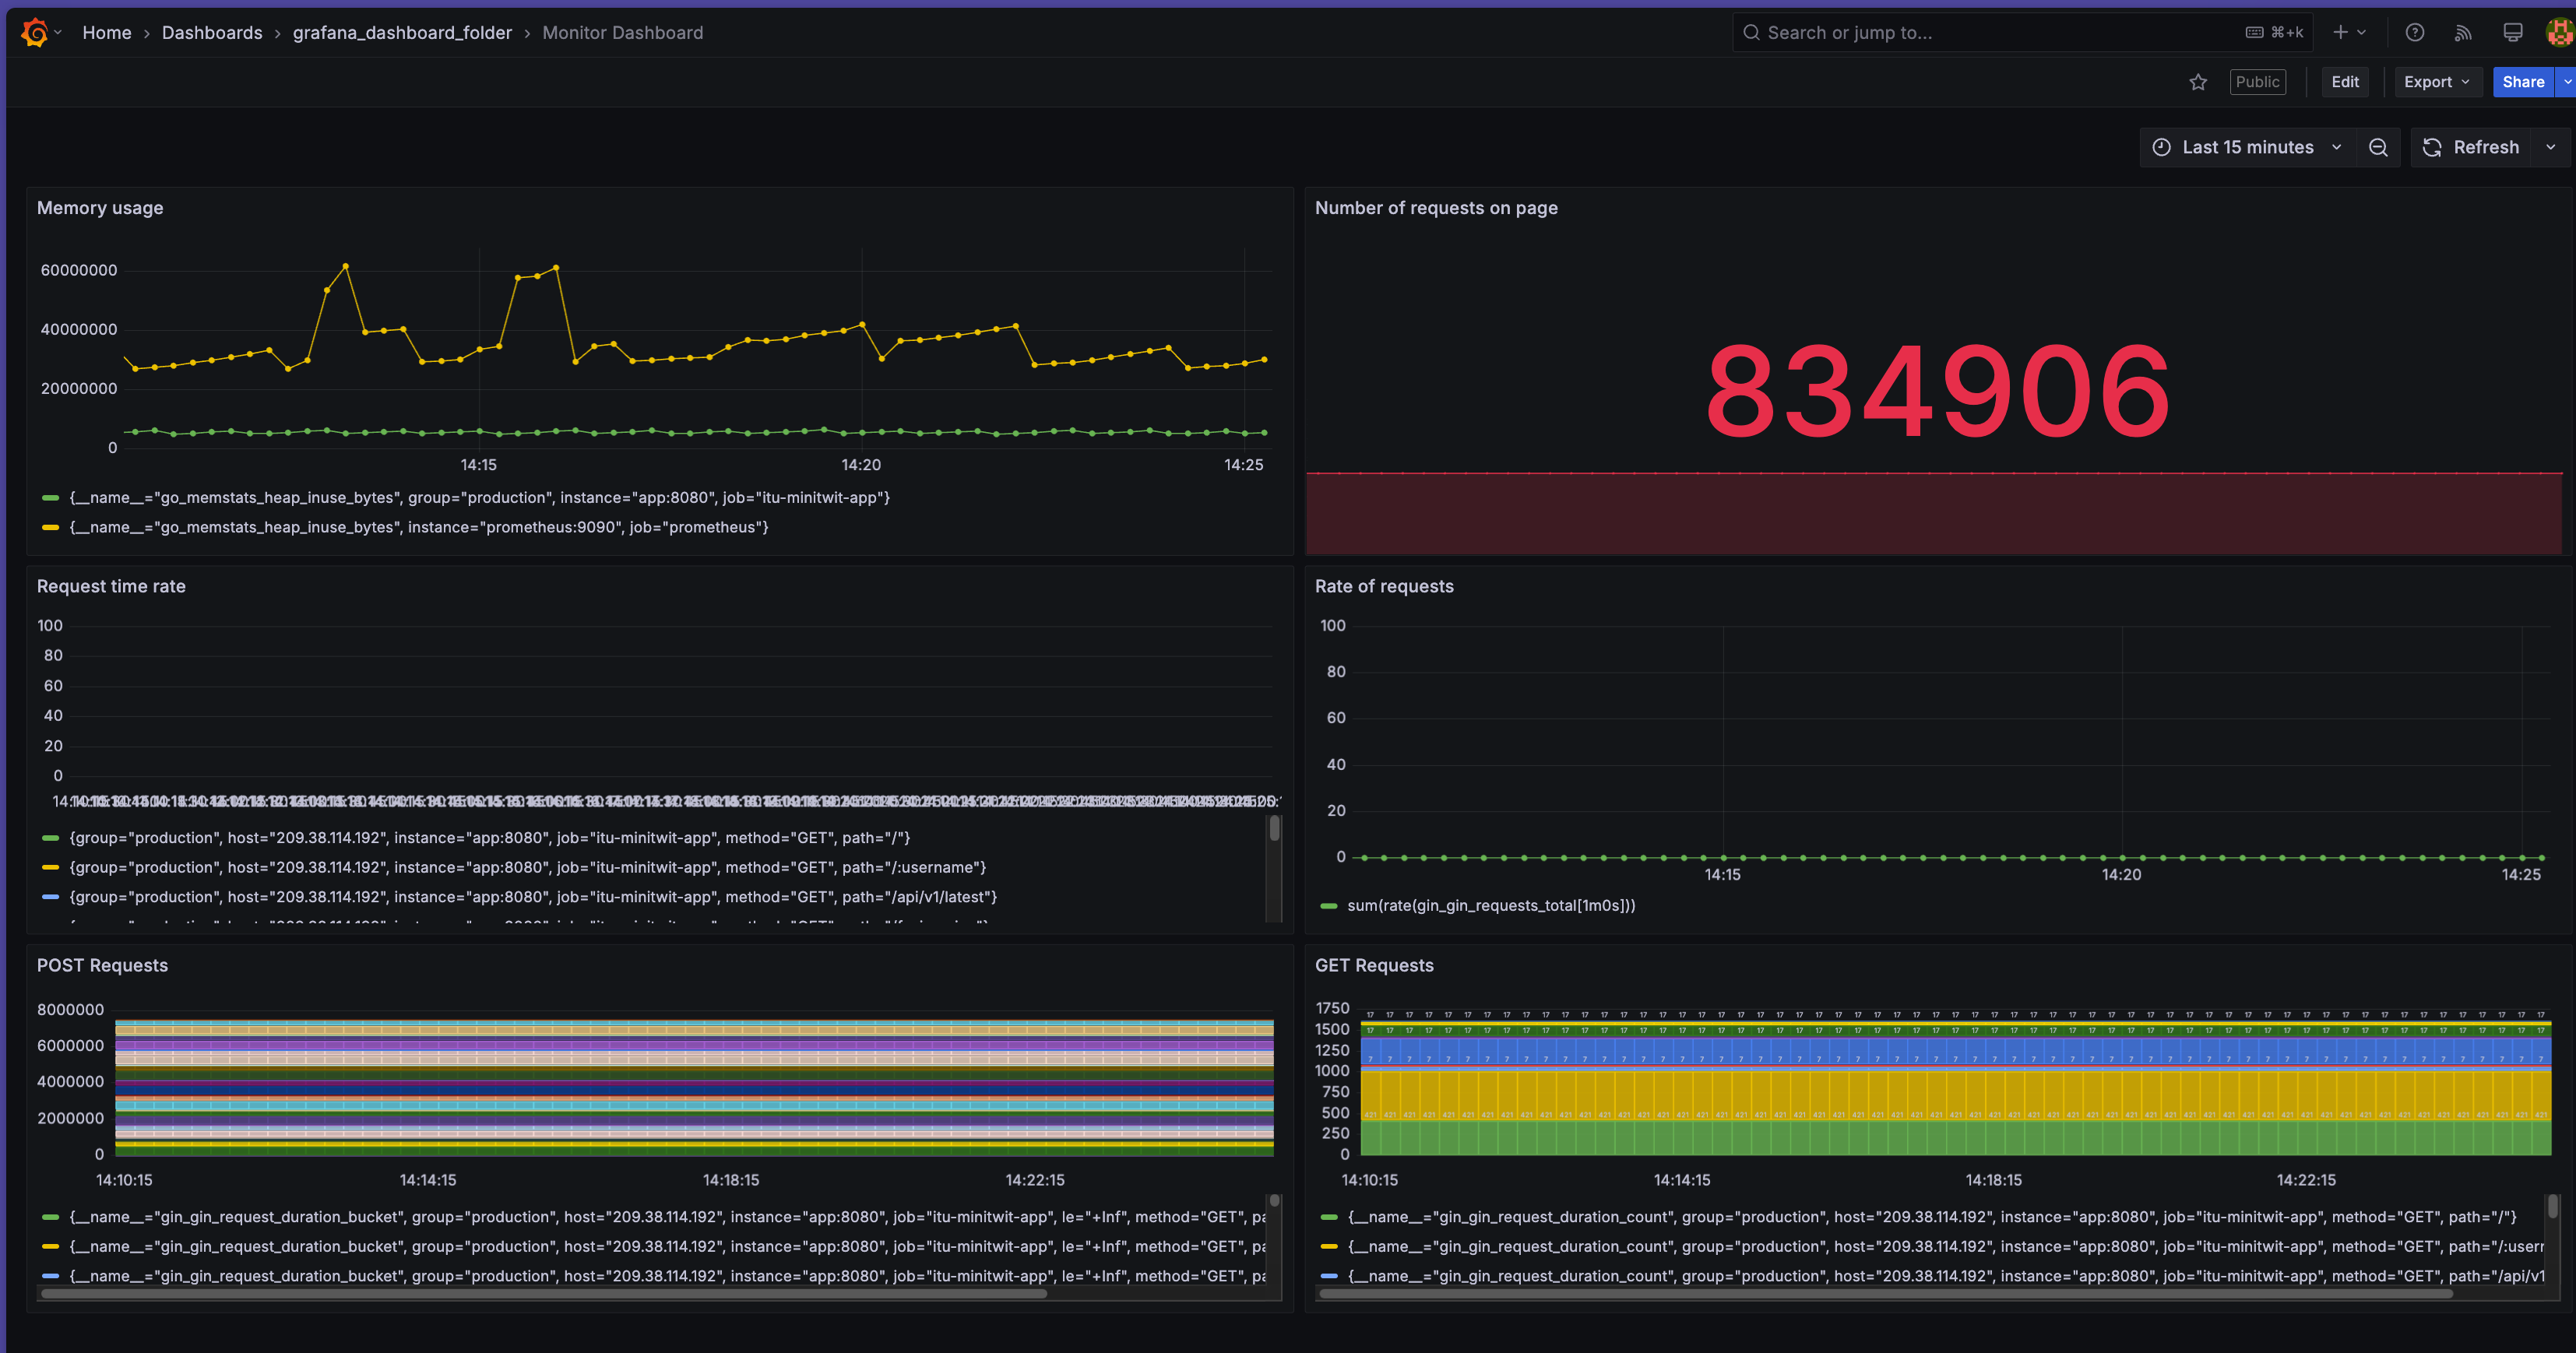
\includegraphics[width=1\linewidth]{images/Monitor.png}
    \caption{The monitoring dashboard, showcasing the number of requests being made, on which endpoints, and their frequency}
    \label{fig:monitor}
\end{figure}

\subsubsection{Logging}
Our logging setup has been based around Grafana Loki as a log aggregation tool, and Grafana Alloy as the log collection tool. Our logging efforts were divided among our Docker containers, reading their respective logs. We decided to split up the dashboard, such that we could see the logs for each Docker container, as observed in figure \ref{fig:logging}. In addition to this, we implemented logs for our MiniTwit application using the standard logging library in Go \texttt{slog}. Here we focused on implementing log events for all of our event handlers providing using different log levels to signify the nature of the problem.

\begin{figure} [H]
    \centering
    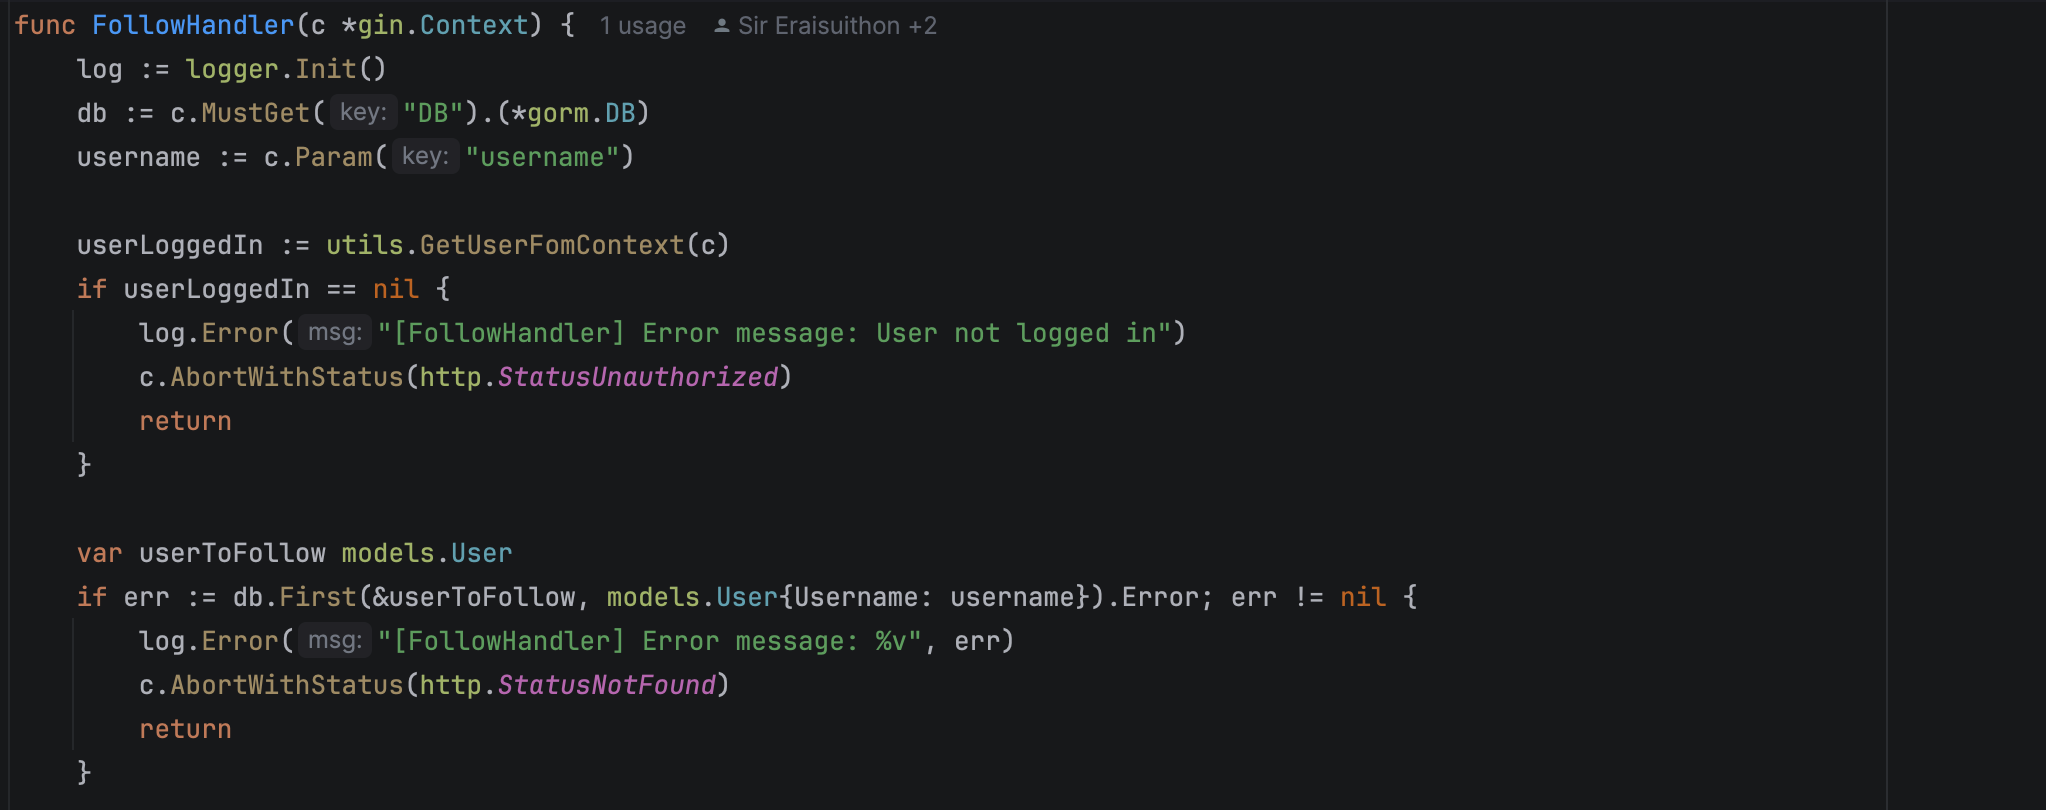
\includegraphics[width=1\linewidth]{images/StdLog.png}
    \caption{Example of logging with FollowHandler showcasing how errors are propagated as a log.}
    \label{fig:enter-label}
\end{figure}
\begin{figure} [H]
    \centering
    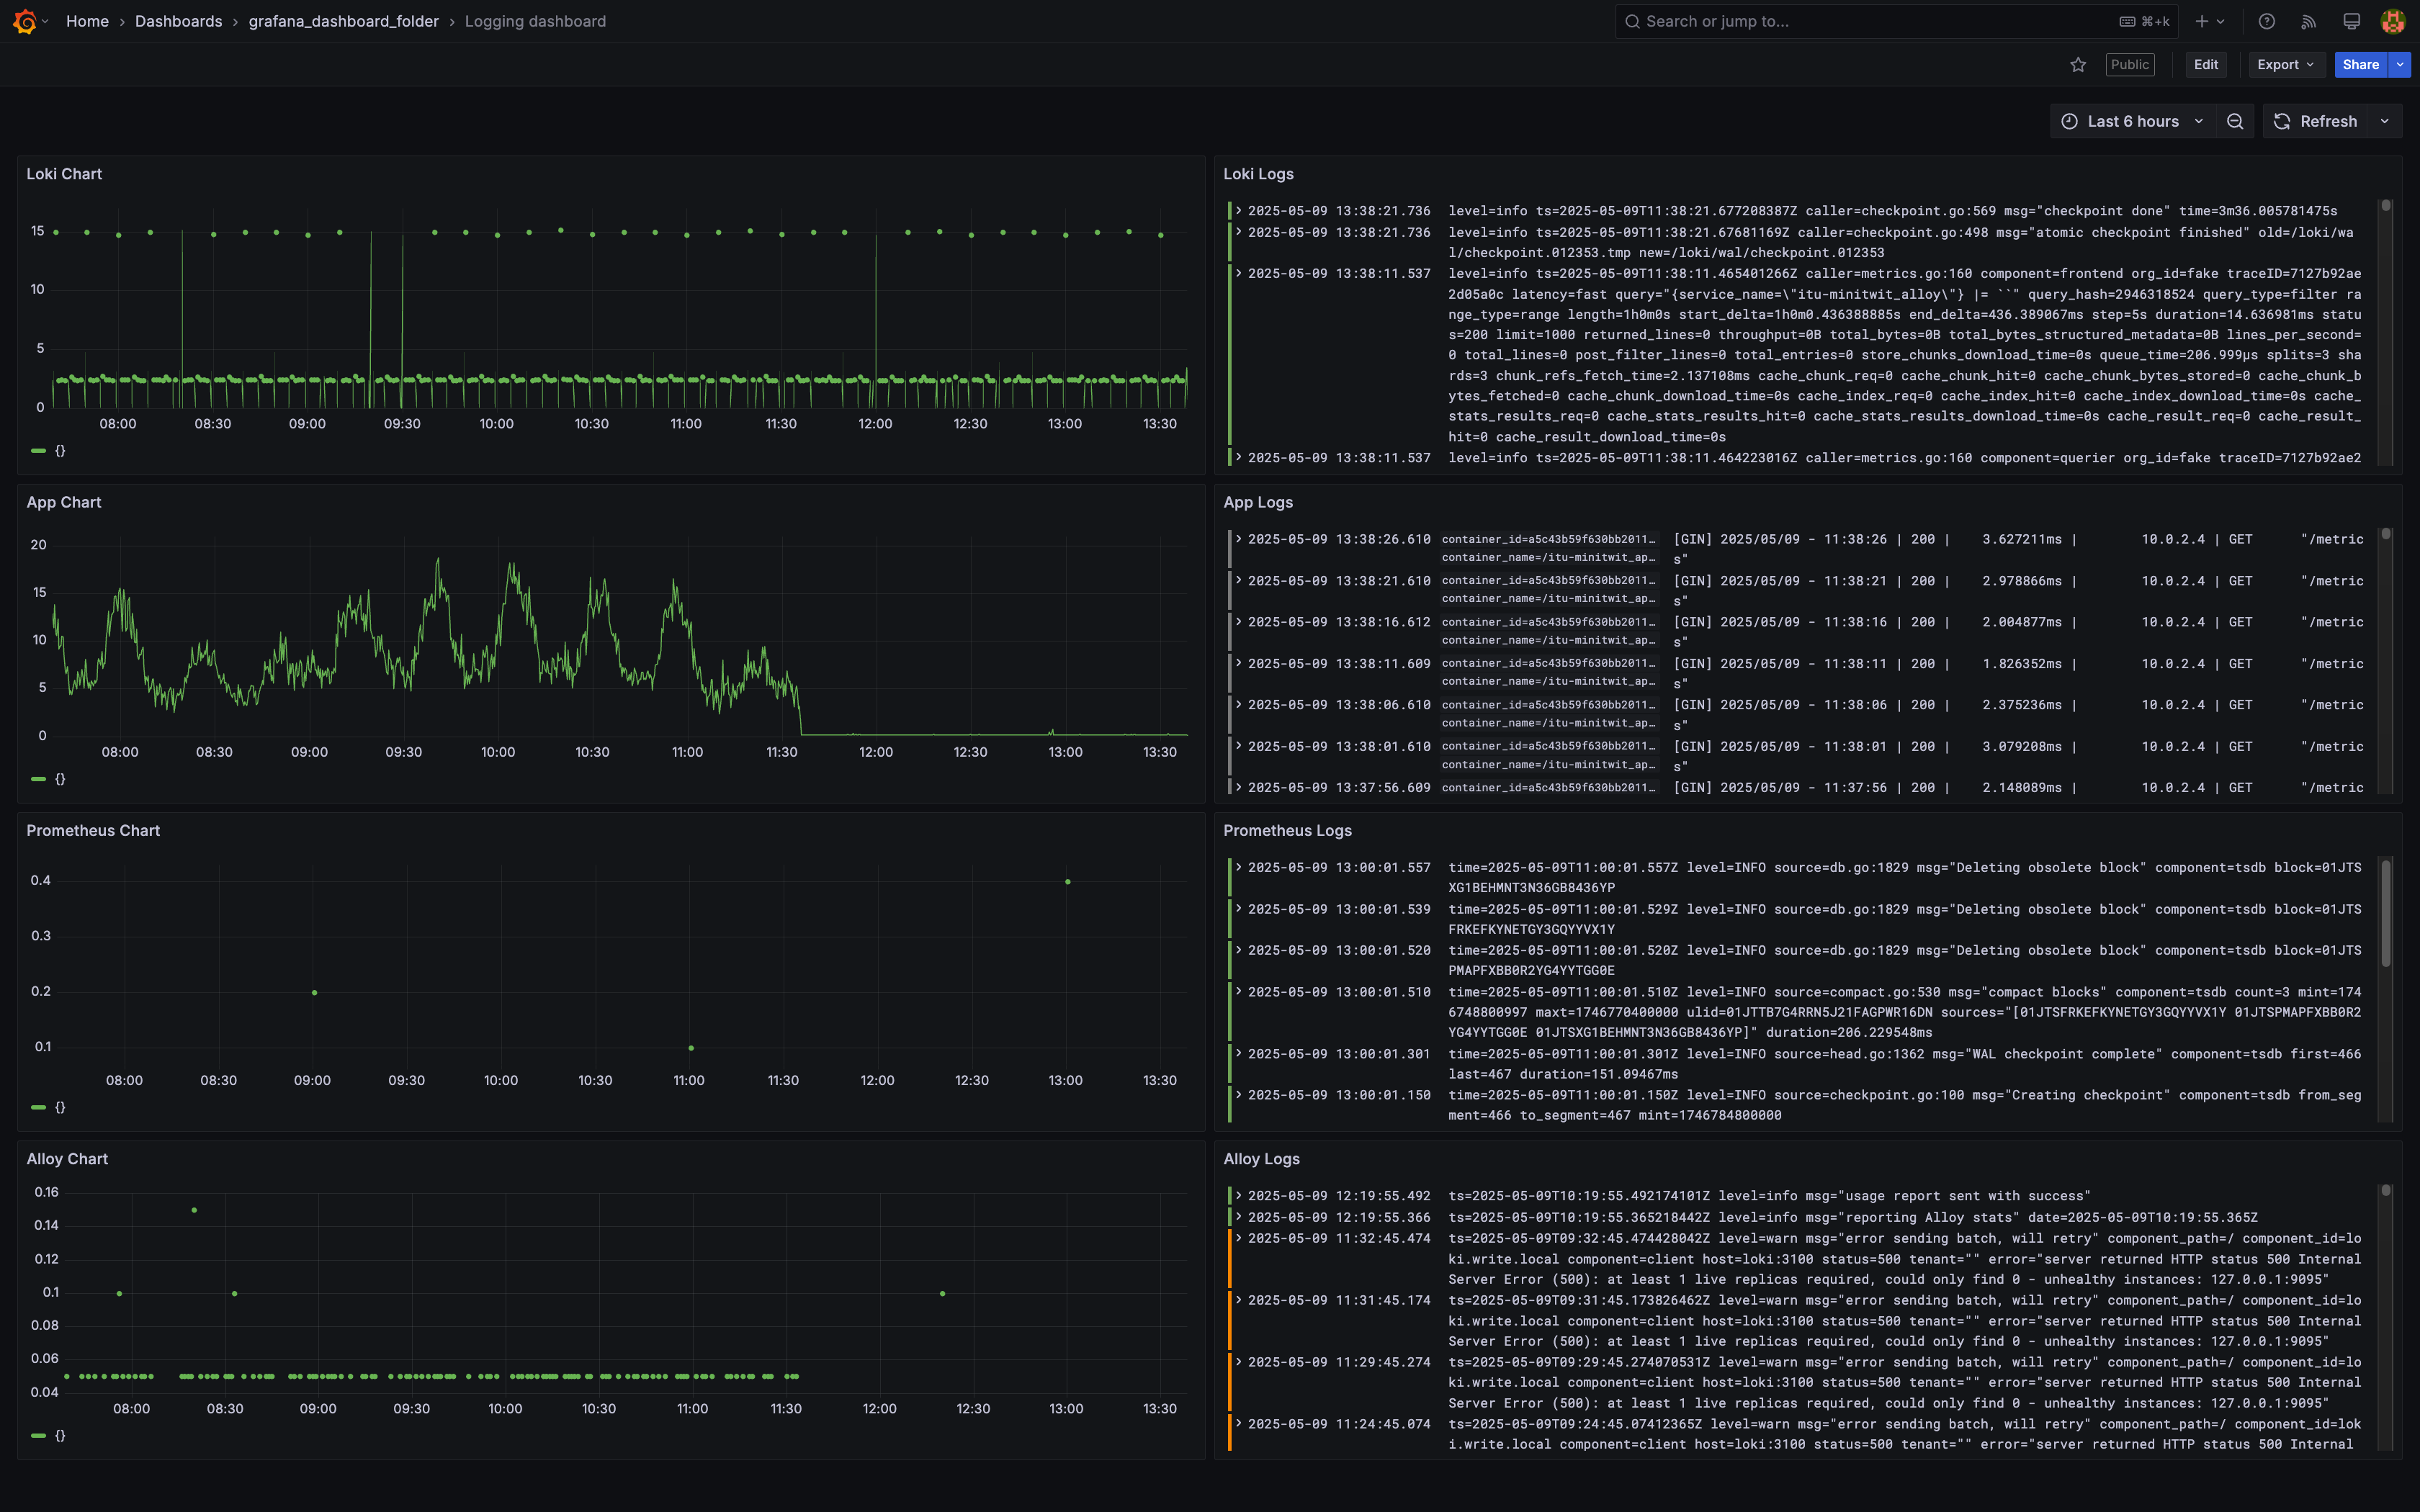
\includegraphics[width=1\linewidth]{images/logging.png}
    \caption{Logging dashboard, showcasing the events by Docker containers}
    \label{fig:logging}
\end{figure}

\subsection{Security assessment}
To identify possible attack surfaces, we made a full port-scan of our server with nmap, which came up with the following open ports;
\begin{description}
    \item[22] SSH into droplet
    \item[80, 443] MiniTwit through traefik
    \item[3000] Grafana
    \item[3100] Loki
    \item[12345] Alloy
    \item[9090] Prometheus
\end{description}
We reasoned that the following were already secure: SSH, MiniTwit, Grafana, and Prometheus. That left Loki and Alloy, where data could be extracted without requiring any form of authentication, which can be seen in table \ref{tab:risk-matrix}. 
\begin{table}[h!]
\centering
\begin{tabular}{|l|lll|}
\hline
\textbf{Risk}   & \multicolumn{3}{c|}{\textbf{Likelyhood}}                                                                    \\ \hline
       & \multicolumn{1}{c|}{Low}                 & \multicolumn{1}{c|}{Medium} & \multicolumn{1}{c|}{High} \\ \hline
Low    & \multicolumn{1}{l|}{MiniTwit}             & \multicolumn{1}{l|}{}       &                           \\ \hline
Medium & \multicolumn{1}{l|}{} & \multicolumn{1}{l|}{Grafana, Prometheus}       & Loki, Alloy               \\ \hline
High   & \multicolumn{1}{l|}{SSH}                 & \multicolumn{1}{l|}{}       &                           \\ \hline
\end{tabular}
\caption{Risk matrix}
\label{tab:risk-matrix}
\end{table}

Our solution to this was to stop exposing the ports for Loki and Alloy, as they are on an internal network in the Docker Swarm, and all relevant data from them can be obtained through Grafana, where authentication is required.

The reason our database does not show up as a potential attack surface is that it is running inside a VPC without public internet access, such that only our application has access to it.
\subsection{Scaling strategy}
Our project implements a containerized architecture using Docker Swarm for orchestration, with a setup that provides several key scalability advantages:

\textbf{Container Orchestration with Docker Swarm}
    \begin{itemize}
        \item All the services are deployed as a Docker stack, configured in a single \texttt{docker-compose} file, which allows for declarative configuration and simplified management
        \item Docker Swarm provides built-in service discovery, load balancing, and rolling updates
        \item The current configuration maintains 3 replicas of the main application to support high availability, redundancy, and rolling updates
    \end{itemize}

The Docker swarm cluster currently consists of just a single node, because additional nodes are not necessary at the current load levels, the load on the server reaching only 15\% of the capacity, as can be seen in figure \ref{fig:cpu_usage}, even at the highest levels of load from the simulator.
 \begin{figure}
    \centering
    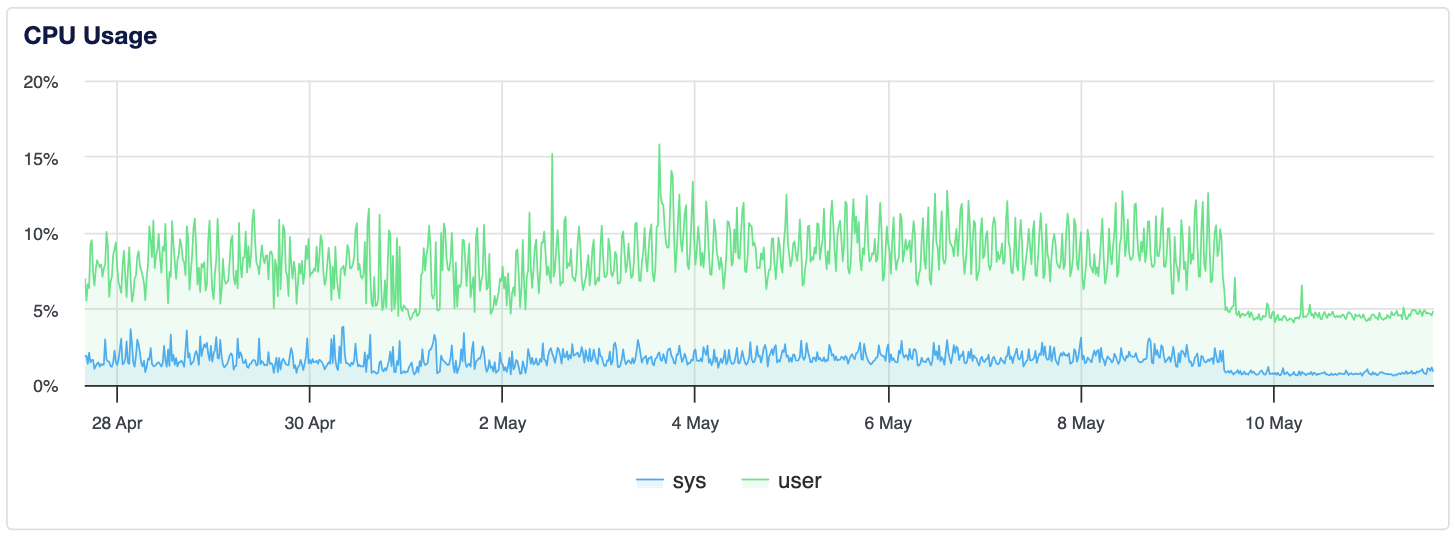
\includegraphics[width=1\linewidth]{images/CPU-Usage.png}
    \caption{VM CPU Usage graph}
    \label{fig:cpu_usage}
\end{figure}
For the database, we made the choice to use Digital Ocean's managed database service, which provides a fully managed PostgreSQL database. This choice was made to simplify database management and ensure high availability and scalability. The managed offering from Digital Ocean allows us to offload the database administration tasks and has built-in scalability and reliability capabilities, such as:

        \begin{itemize}
            \item Adding standby nodes for high availability
            \item Deploying read-only nodes for scaling read operations
            \item Automated backups and point-in-time recovery
        \end{itemize}


The architecture we've implemented provides flexible scaling capabilities through both vertical and horizontal approaches. Vertical scaling can be achieved by upgrading to more powerful VM instances with increased CPU, memory, and storage resources. For horizontal scaling, Docker Swarm's orchestration allows us to seamlessly add additional nodes to the cluster and increase the application replica count. At the same time, Digital Ocean's managed PostgreSQL service enables horizontal read scaling through read-only database nodes. This dual-scaling capability creates a robust foundation for future enhancements, including automated scaling based on load metrics and multi-region deployments for improved global performance and redundancy. Our infrastructure design emphasizes scalability as a core principle, ensuring the system can efficiently adapt to growing demands without significant architectural changes.

\subsection{Use of Artificial Intelligence}
In our project, we have used Anthropic’s artificial intelligence tool \textit{Claude} \parencite{claude}. Claude has been helpful when it came to adopting new technologies and frameworks that none of us had worked with prior. A major concern however, has been that Claude often times seems to miss the broader context, we are working on, ignores security concerns, and generally tends to overcomplicate its output. As such, while the use of AI has been helpful in providing an understanding of the different components in our project, it has not been able to meaningfully replace the work of us as developers.
